
\begin{figure}[h!]
	\centering
	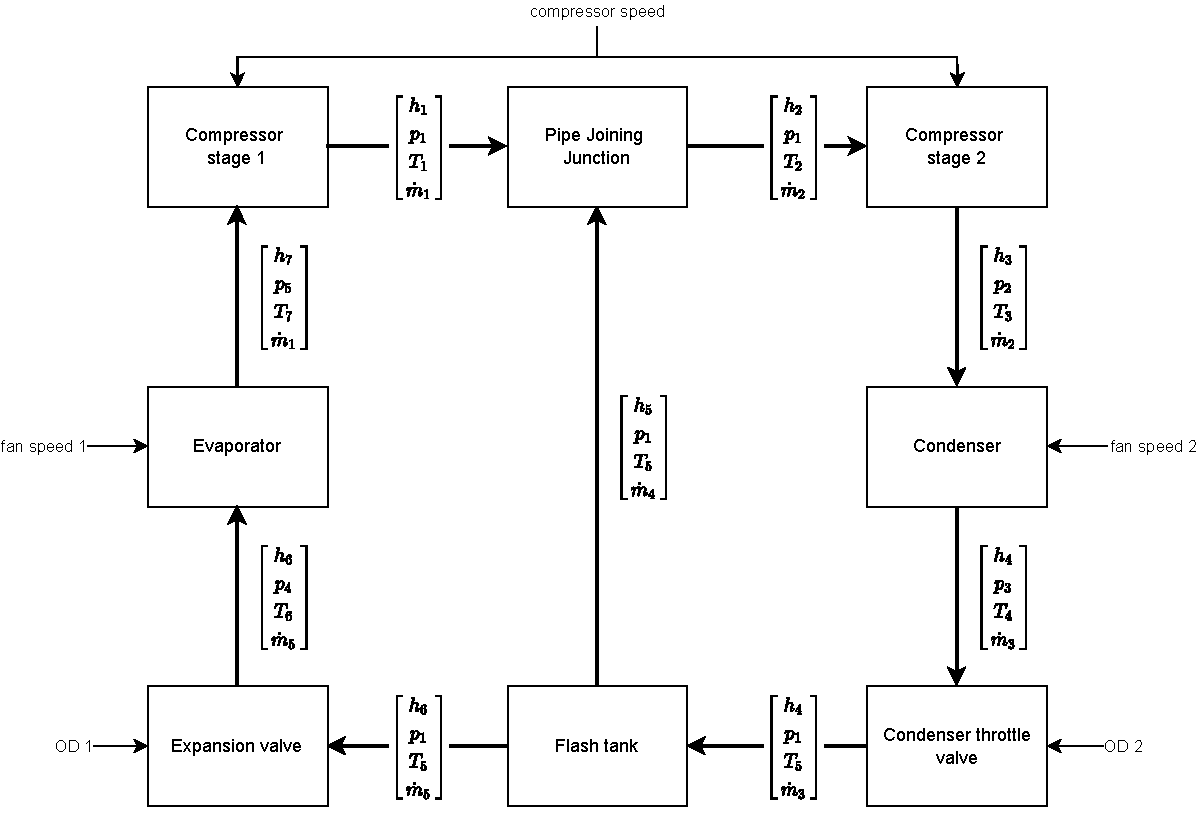
\includegraphics[width=1\textwidth]{Graphics/Block_Diagram.pdf}
	\caption{Initial Block Diagram with states}
	\label{fig:Block_diagram}
\end{figure}

\subsubsection{State variables}

Through the component model section the behavior of the system components was described. Due to the large variance in the dynamic speed of the system parameters, the fast variables were defined algebraically, while the slow dynamics were modelled with differential equations. \\
While including the dynamics of the faster parameters would yield a potentially more accurate model, it is unnecessary from a control point of view, as this model is intended for control of the slow dynamics. In addition, the added accuracy will likely be unnoticable due to various uncertanties in the model. The specific decision of which parameters to model dynamically is heavily inspired by previous work \cite{Sorensen2013}.\\
The parameters described with differential equations are the system states. The differential equations are collected and put in vector form in \cref{eq:f_noSub}. The function $f(x,u)$ is thus the nonlinear model of the system. It contains 11 states, 5 control inputs and 1 disturbance. 


\begin{equation} \label{eq:f_noSub} \renewcommand{\arraystretch}{2.4}
	f(x,u) =  \dfrac{d}{dt} \begin{bmatrix}
		M_{pjj}			\\				%pjj
		M_{con} 		\\				%condenser
		T_m 			\\				%condenser
		\dot{m}_{air}	\\				%evaporator
		T_{ml}			\\				%evaporator
		T_{mv}			\\				%evaporator
		M_l				\\				%evaporator
		M_v				\\				%evaporator
		T_{air}			\\				%box
		T_{box}			\\				%box
		T_{cargo}		\\				%box
		
	\end{bmatrix}
	=
	\begin{bmatrix}
		\dot{m}_1 + \dot{m}_4 - \dot{m}_2 \\										%pjj
		\dot{m}_{2} - \dot{m}_{3}	\\												%condenser
		\dfrac{Q_{rm} - Q_{ma}}{M_m \cdot Cp_m} \\									%condenser
		\dfrac{\bar{\dot{m}}_{air}  - \dot{m}_{air}} {10s}		\\					%evaporator
		\dfrac{Q_{aml}-Q_{ml} + Q_{mvml}}{M_m \cdot Cp_m \cdot \sigma}        \\	%evaporator
		\dfrac{Q_{amv} - Q_{mv} - Q_{mvml}}{M_m \cdot Cp_m \cdot (1- \sigma)}	\\	%evaporator
		\dot{m}_{5} - \dot{m}_{lv}		\\											%evaporator
		\dot{m}_{lv} - \dot{m}_{1}	\\												%evaporator
		\dfrac{Q_{ca} + Q_{ba} + Q_{fan} -Q_{cool}}{M_{air} \cdot Cp_{air}} \\		%box
		\dfrac{Q_{amb} - Q_{ba}}{M_{box} \cdot Cp_{box}} \\							%box
		\dfrac{-Q_{ca}}{M_{cargo} \cdot Cp_{cargo}}									%box
	\end{bmatrix}	
\end{equation}






\begin{equation} \label{eq:f_Sub} \renewcommand{\arraystretch}{3.4}
	f(x,u) =   \dfrac{d}{dt} \begin{bmatrix}
		M_{_{PJJ}}		\\				%pjj
		M_{Con} 		\\				%condenser
		T_m 			\\				%condenser
		\dot{m}_{air}	\\				%evaporator
		T_{ml}			\\				%evaporator
		T_{mv}			\\				%evaporator
		M_l				\\				%evaporator
		M_v				\\				%evaporator
	\end{bmatrix}
	=
	\begin{bmatrix}
		\left(\dfrac{V_1}{v_{1_{COM1}}} - \dfrac{V_C}{v_{2_{COM1}}}\right) \dfrac{\omega}{2} + \dfrac{\dot{m}_{3} \cdot h_4 - \dot{m}_{5} \cdot h_6}{h_5} - \left(\dfrac{V_1}{v_{1_{COM2}}} - \dfrac{V_C}{v_{2_{COM2}}}\right) \dfrac{\omega}{2} \\										%pjj
		\left(\dfrac{V_1}{v_{1_{COM2}}} - \dfrac{V_C}{v_{2_{COM2}}}\right) \dfrac{\omega}{2} - f_p(\Theta_1) \cdot K  \sqrt{\dfrac{1}{v_{_{CTV_{in}}}} (p_{3} - p_{1})}	\\												%condenser
		\dfrac{U A_{rm} \cdot (T_r - T_m) - U A_{ma} \cdot (T_m - T_{ambi})\cdot \left(0.05 + \dfrac{U_{fan_1}}{1530}\right)}{M_m \cdot Cp_m} \\									%condenser
		\dfrac{\left( 0.7273 + 0.1202 \cdot U_{*_{\dot{m}}}  -0.0044 \cdot	U_{*_{\dot{m}}}^2 \right) \cdot \rho_{air}  - \dot{m}_{air}} {10s}		\\					%evaporator
		\dfrac{Cp_{air} \cdot \dot{m}_{air} \cdot (T_{retsh} - T_{ml})-U A_1 \cdot (T_{ml} - T_l) \cdot \sigma + U A_3 \cdot (T_{mv} - T_{ml})}{M_m \cdot Cp_m \cdot \sigma}        \\	%evaporator
		\dfrac{Cp_{air} \cdot \dot{m}_{air} \cdot (T_{retfan} - T_{mv}) - U A_2 \cdot (T_{mv} - T_v) \cdot (1- \sigma) - U A_3 \cdot (T_{mv} - T_{ml})}{M_m \cdot Cp_m \cdot (1- \sigma)}	\\	%evaporator
		f_p(\Theta_2) \cdot K  \sqrt{\dfrac{1}{v_{_{EV_{in}}}} (p_{1} - p_{4})} - \dfrac{U A_1 \cdot (T_{ml} - T_l) \cdot \sigma}{h_{dew} - h_{6}}		\\											%evaporator
		\dfrac{U A_1 \cdot (T_{ml} - T_l) \cdot \sigma}{h_{dew} - h_{6}} - \left(\dfrac{V_1}{v_{1_{COM1}}} - \dfrac{V_C}{v_{2_{COM1}}}\right) \dfrac{\omega}{2}	\\												%evaporator
	\end{bmatrix}
\end{equation}





\begin{equation} \label{eq:Gpjj}\renewcommand{\arraystretch}{2.5}
	g_{_{PJJ}}(x,u) =  \begin{bmatrix}
		h_{2}				\\ %pjj
		\dot{m}_{2}			\\ %pjj
	\end{bmatrix}
	-
	\begin{bmatrix}
		\dfrac{h_{1} \cdot \dot{m}_{1} + h_{5} \cdot \dot{m}_{4}}{ \dot{m}_{2} } \\ 	%pjj
		\dot{m}_{1} + \dot{m}_{4} \\													%pjj
	\end{bmatrix}
	=\textbf{0}
\end{equation}


\begin{equation} \label{eq:Gcs2}\renewcommand{\arraystretch}{2.5}
	g_{_{COM2}}(x,u) =  \begin{bmatrix}
		\dot{m}_2  		 	\\ %COM2
		h_{3}				\\ %COM2
		v_{1_{COM2}}			\\ %COM2
		v_{2_{COM2}}			\\ %COM2
		p_{i1_{COM2}}		\\ %COM2
		p_{i2_{COM2}}		\\ %COM2
		\gamma				\\ %COM2
		T_{3}				\\ %COM2
	\end{bmatrix}
	-
	\begin{bmatrix}
		\left(\dfrac{V_1}{v_{1_{COM2}}} - \dfrac{V_C}{v_{2_{COM2}}}\right) \dfrac{\omega}{2} \\			%COM2
		\Upsilon(T_{3}, p_{2})		\\													%COM2
		\Gamma(T_{2},p_{i1_{COM2}}) \\													%COM2
		\left(\dfrac{p_{i2_{COM2}}}{p_{i1_{COM2}}}\right)^{\frac{-1}{\gamma}} \\		%COM2
		p_{1} - kl_1 \cdot \omega \\													%COM2
		p_{2} + kl_2 \cdot \omega \\													%COM2
		\dfrac{C_{cp}}{C_{cv}} \\														%COM2
		T_{2}\cdot \left(\dfrac{p_{2}}{p_{1}}\right)^{\frac{\gamma-1}{\gamma}}	\\		%COM2
	\end{bmatrix}
	=\textbf{0}
\end{equation}


\begin{equation} \label{eq:Gcondenser}\renewcommand{\arraystretch}{2.5}
	g_{_{Con}}(x,u) =  \begin{bmatrix}
		h_{4}				\\ %condenser
		p_{2}				\\ %condenser
		\dot{m}_{3}			\\ %condenser
		Q_{rm}				\\
		Q_{ma}				\\
	\end{bmatrix}
	-
	\begin{bmatrix}
		h_{3} - \dfrac{Q_{rm}}{\dot{m}_{2}}	\\											%condenser
		p_{3} - \lambda \cdot \dot{m}_{2}			\\									%condenser
		\dot{m}_{2} + \dfrac{M_{con} - \frac{V_i}{v_{Con}}}{1s}	\\						%condenser
		U A_{rm} \cdot (T_r - T_m) \\
		U A_{ma} \cdot (T_m - T_{ambi})\cdot \left(0.05 + \dfrac{U_{fan_1}}{1530}\right) \\
	\end{bmatrix}
	=\textbf{0}
\end{equation}




\begin{equation} \label{eq:Gvalves}\renewcommand{\arraystretch}{2.5}
	g_{_{Val}}(x,u) =  \begin{bmatrix}
		\dot{m}_{3}			\\ %condenser valve

		\dot{m}_{5}			\\ %expansion valve
	\end{bmatrix}
	-
	\begin{bmatrix}
		f_p(\Theta_1) \cdot K  \sqrt{\dfrac{1}{v_{_{CTV_{in}}}} (p_{3} - p_{1})}\\		%condenser valve
		f_p(\Theta_2) \cdot K  \sqrt{\dfrac{1}{v_{_{EV_{in}}}} (p_{1} - p_{4})}\\			%expansion valve
	\end{bmatrix}
	=\textbf{0}
\end{equation}

\begin{equation} \label{eq:Gflashtank}\renewcommand{\arraystretch}{2.5}
	g_{_{FT}}(x,u) =  \begin{bmatrix}
		\dot{m}_{4}			\\
		\dot{m}_{5}				\\
		h_{5}  \\
		h_{6} \\
	\end{bmatrix}
	-
	\begin{bmatrix}
		\dfrac{\dot{m}_{3} \cdot h_4 - \dot{m}_{5} \cdot h_6}{h_5}					\\
		\dot{m}_{3} - \dot{m}_{4}					\\
		N(p_1)\\
		M(p_1)\\
	\end{bmatrix}
	=\textbf{0}
\end{equation}



\begin{equation} \label{eq:Gevaporator}\renewcommand{\arraystretch}{2.5}
	g_{_{Eva}}(x,u) =  \begin{bmatrix}
		\sigma		\\
		T_{retfan}	\\
		T_{retsh}	\\
		U_{*_P}	\\
		Q_{fan_2}		\\
		Q_{amv}		\\
		Q_{aml}		\\
		U_{*_{\dot{m}}}	\\
		\bar{\dot{V}}_{air}		\\
		\bar{\dot{m}}_{air}		\\
		Q_{mvml}	\\
		Q_{ml}		\\
		Q_{mv}		\\
		p_{5}		\\
		h_{lv}			\\
		h_v 		\\
		T_{sup}		\\
		\dot{m}_{lv}\\
	\end{bmatrix}
	-
	\begin{bmatrix}
		\dfrac{M_l \cdot v_{_{Eva}}}{V_i}							\\
		T_{ret} + \dfrac{Q_{fan_2}}{\dot{m}_{air} \cdot Cp_{air}}			\\
		T_{retfan} - \dfrac{Q_{amv}}{\dot{m}_{air} \cdot Cp_{air}}		\\
		\left( \dfrac{U_{fan_2}}{3060}\cdot 100 - 55.56 \right) \cdot 0.0335 \\
		177.76 + 223.95 \cdot U_{*_P} + 105.85 \cdot U_{*_P}^2 + 16.74 \cdot U_{*_P}^3 \\
		Cp_{air} \cdot \dot{m}_{air} \cdot (T_{retfan} - T_{mv}) 	 \\
		Cp_{air} \cdot \dot{m}_{air} \cdot (T_{retsh} - T_{ml}) \\
		(U_{fan_2} - 2270.4)\cdot 0.0017 \\
		0.7273 + 0.1202 \cdot 	U_{*_{\dot{m}}}  -0.0044 \cdot	U_{*_{\dot{m}}}^2\\
		\bar{\dot{V}}_{air} \cdot \rho_{air}	\\
		U A_3 \cdot (T_{mv} - T_{ml})	\\
		U A_1 \cdot (T_{ml} - T_l) \cdot \sigma	\\
		U A_2 \cdot (T_{mv} - T_v) \cdot (1- \sigma)	\\
		\Pi \left( h_v, \dfrac{V_i-V_l}{M_v} \right)		\\
		h_{6} + \dfrac{Q_{ml}}{\dot{m}_{5}}			\\
		h_{dew} + \dfrac{Q_{mv}}{\dot{m}_{lv}}   		\\
		T_{retfan} +  \dfrac{Q_{aml} + Q_{amv}}{Cp_{air} \cdot \dot{m}_{air}} \\
		\dfrac{Q_{ml}}{h_{dew} - h_{6}}		\\
	\end{bmatrix}
	=\textbf{0}
\end{equation}



\begin{equation} \label{eq:Gcs1}\renewcommand{\arraystretch}{2.5}
	g_{_{COM1}}(x,u) =  \begin{bmatrix}
		\dot{m}_1  		 	\\ %COM1
		h_{1}				\\ %COM1
		v_{1_{COM1}}			\\ %COM1
		v_{2_{COM1}}			\\ %COM1
		p_{i1_{COM1}}		\\ %COM1
		p_{i2_{COM1}}		\\ %COM1
		\gamma				\\ %COM1
		T_{1}				\\ %COM1
	\end{bmatrix}
	-
	\begin{bmatrix}
		\left(\dfrac{V_1}{v_{1_{COM1}}} - \dfrac{V_C}{v_{2_{COM1}}}\right) \dfrac{\omega}{2} \\			%COM1
		\Upsilon(T_{1}, p_{1})		\\													%COM1
		\Gamma(T_{7},p_{i1_{COM1}}) \\													%COM1
		\left(\dfrac{p_{i2_{COM1}}}{p_{i1_{COM1}}}\right)^{\frac{-1}{\gamma}} \\		%COM1
		p_{5} - kl_1 \cdot \omega \\													%COM1
		p_{1} + kl_2 \cdot \omega \\													%COM1
		\dfrac{C_{cp}}{C_{cv}} \\												%COM1
		T_{7}\cdot \left(\dfrac{p_{1}}{p_{5}}\right)^{\frac{\gamma-1}{\gamma}}	\\		%COM1
	\end{bmatrix}
	=\textbf{0}
\end{equation}


\begin{equation} \label{eq:Gbox}\renewcommand{\arraystretch}{2.5}
	g_{_{Box}}(x,u) =  \begin{bmatrix}
		Q_{cool}		\\ %box
		Q_{amb}			\\ %box
		Q_{ba}			\\ %box
		Q_{ca}			\\ %box
	\end{bmatrix}
	-
	\begin{bmatrix}
		Cp_{air} \cdot \dot{m}_{air} \cdot (T_{ret} - T_{sup})  \\	%box
		(T_{ambi} - T_{box}) \cdot U A_{amb} 					\\	%box
		(T_{box} - T_{air}) \cdot U A_{ba} 						\\	%box
		(T_{cargo} - T_{air}) \cdot U A_{ca}				 	\\	%box
	\end{bmatrix}
	=\textbf{0}
\end{equation}





\begin{equation} \label{eq:Gtotal}\renewcommand{\arraystretch}{2.5}
	g(x,u) =  \begin{bmatrix}
		g_{_{PJJ}}(x,u)  		 	\\ %COM1
		g_{_{COM2}}(x,u)				\\ %COM1
		g_{_{Con}}(x,u)			\\ %COM1
		g_{_{Val}}(x,u)			\\ %COM1
		g_{_{FT}}(x,u)		\\ %COM1
		g_{_{Eva}}(x,u)		\\ %COM1
		g_{_{COM1}}(x,u)			\\
		g_{_{Box}}(x,u)			\\
	\end{bmatrix}
	= \textbf{0}
\end{equation}



